\newcommand{\tikzunderarrowA}{
	\tikzset{external/export next=false}
	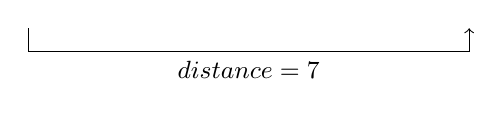
\begin{tikzpicture}
	\draw [->] (0, 0) -- ++(0, -0.3) -- node[midway, below] {\small $distance = 7$} ++(5.6, 0) -- ++(0, 0.3);
	\end{tikzpicture}
}

\newcommand{\tikzunderarrowB}{
	\tikzset{external/export next=false}
	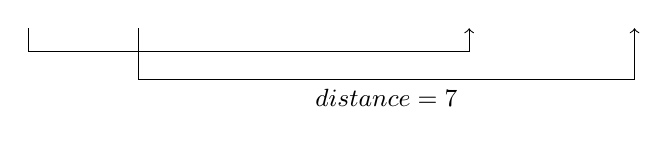
\begin{tikzpicture}
	\draw [->] (0, 0) -- ++(0, -0.3) -- ++(5.6, 0) -- ++(0, 0.3);
	\draw [->] (1.4, 0) -- ++(0, -0.65) -- node[midway, below] {\small $distance = 7$} ++(6.3, 0) -- ++(0, 0.65);
	\end{tikzpicture}
}

\begin{enumerate} \nosep
	\item $insert\ length = 7,\ copy\ length = 5,\ distance = 7$
	\\[5pt]
	$\begin{array}{|*{13}{f{2ex}|}}
	\cline{1-7} \cline{9-13}
	w & o & r & d & s & , & \texttt{\textvisiblespace} & $\cdot$ & w & o & r & d & s \fixcline
	\cline{1-7} \cline{9-13}
	\end{array}$
	\\[1pt]
	\trimbox{-0.5ex 0.3ex 0 0}{\tikzunderarrowA}
\end{enumerate}

\begin{enumerate} \nosep
	\item $insert\ length = 7,\ copy\ length = 2,\ distance = 7$
	\item $insert\ length = 0,\ copy\ length = 3,\ distance = 7$ (always the same distance)
	\\[5pt]
	$\begin{array}{|*{14}{f{2ex}|}l}
	\cline{1-7} \cline{9-10} \cline{12-14}
	w & o & r & d & s & , & \texttt{\textvisiblespace} & $\cdot$ & w & o & $\cdot$ & r & d & s \fixcline
	\cline{1-7} \cline{9-10} \cline{12-14}
	\end{array}$
	\\[1pt]
	\trimbox{-0.5ex 1.5ex 0 0}{\tikzunderarrowB}
\end{enumerate}